	Мальчик наблюдает за движущимися относительно него фонарями и деревьями, имея ограниченный угол зрения.
На рисунке представлено, что он видит из окна на примере фонарей. При движении каждый фонарь перемещается от левого края угла зрения к правому. Разумно считать фонарь тогда, когда его столб пересекает правый край. В таком случае один и тот же фонарь не будет учтен несколько раз.
	
\begin{figure}[h!]
	\centering
	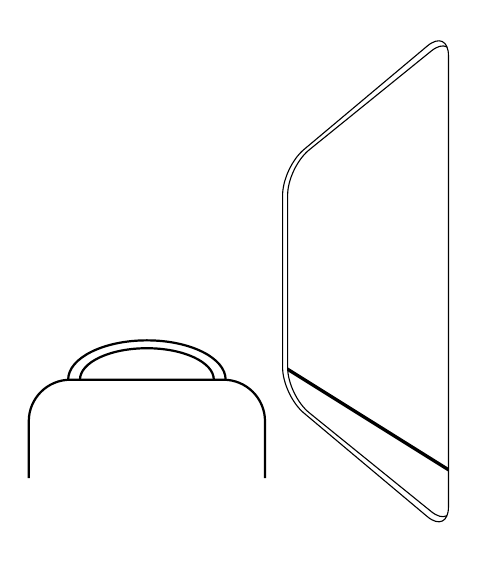
\begin{tikzpicture}[scale = 0.5]
		\draw[thick] (-2, -2.5) arc (180:0:2 and 1);
		\draw[thick] (-1.7, -2.5) arc (180:0: 1.7 and 0.8);
		\draw[thick, rounded corners = 15] (-3, -5) -- (-3, -2.5) -- (3, -2.5) -- (3, -5); 
		\draw[rounded corners = 10] (-40:4.5) -- (-40:10) -- (40:10) -- (40:4.5) -- cycle;
		\begin{scope}
    			\clip[rounded corners = 10] (-40:4.5) -- (-40:10) -- (40:10) -- (40:4.5) -- cycle;
			\draw[rounded corners = 10] (-39:4.6) -- (-39:10) -- (39:10) -- (39:4.6) -- cycle;
		\end{scope}
		\begin{scope}
    			\clip[rounded corners = 10] (-40:4.5) -- (-40:10) -- (40:10) -- (40:4.5) -- cycle;
			\clip[rounded corners = 10] (-39:4.6) -- (-39:10) -- (39:10) -- (39:4.6) -- cycle;
			\draw[very thick] (-32:0) -- (-32:13);
%			\fill[gray!80] (-32:0) -- (-32:13) -- (-50:13) -- cycle;
%			\fill[green!80!blue!60] (-32:0) -- (-32:13) -- (-15:13) -- cycle;
			\flash{7}{-3}{4}{thick}{0};
			\flash{0.8*7}{-0.8*3}{0.8*4}{thick}{1};
			\flash{0.62*7}{-0.62*3}{0.62*4}{thick}{2};
		\end{scope}
	\end{tikzpicture}
\end{figure}

	Мальчик всегда видит ровно три фонаря. Тогда в тот момент, когда один из фонарей (фонарь $0$) исчезает из поля зрения, в нем должен появляться следующий (фонарь $3$). Иначе существовал бы такой промежуток времени, в котором в угле зрения находилось бы всего два фонаря, а это противоречит условию. 
\begin{figure}[h!]
	\begin{minipage}{0.49\linewidth}
	\centering
	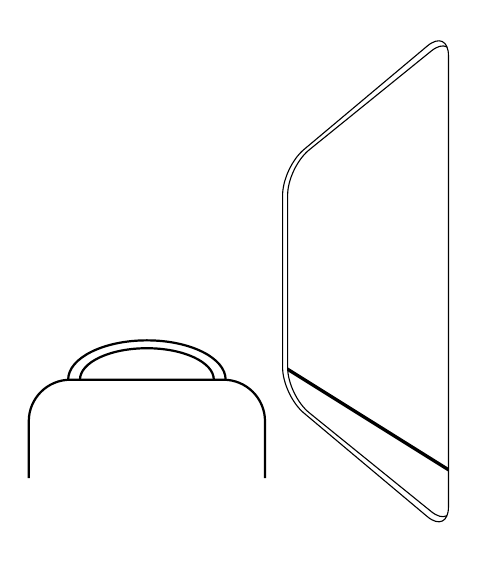
\begin{tikzpicture}[scale = 0.5]
		\draw[thick] (-2, -2.5) arc (180:0:2 and 1);
		\draw[thick] (-1.7, -2.5) arc (180:0: 1.7 and 0.8);
		\draw[thick, rounded corners = 15] (-3, -5) -- (-3, -2.5) -- (3, -2.5) -- (3, -5); 
		\draw[rounded corners = 10] (-40:4.5) -- (-40:10) -- (40:10) -- (40:4.5) -- cycle;
		\begin{scope}
    			\clip[rounded corners = 10] (-40:4.5) -- (-40:10) -- (40:10) -- (40:4.5) -- cycle;
			\draw[rounded corners = 10] (-39:4.6) -- (-39:10) -- (39:10) -- (39:4.6) -- cycle;
		\end{scope}
		\begin{scope}
    			\clip[rounded corners = 10] (-40:4.5) -- (-40:10) -- (40:10) -- (40:4.5) -- cycle;
			\clip[rounded corners = 10] (-39:4.6) -- (-39:10) -- (39:10) -- (39:4.6) -- cycle;
			\draw[very thick] (-32:0) -- (-32:13);
%			\fill[gray!80] (-32:0) -- (-32:13) -- (-50:13) -- cycle;
%			\fill[green!80!blue!60] (-32:0) -- (-32:13) -- (-15:13) -- cycle;
			\flash{1.06*7}{-1.06*3}{1.06*4}{thick}{0};
			\flash{0.85*7}{-0.85*3}{0.85*4}{thick}{1};
			\flash{0.66*7}{-0.66*3}{0.66*4}{thick}{2};
		\end{scope}
	\end{tikzpicture}	
	\end{minipage}
	\begin{minipage}{0.49\linewidth}
	\centering
	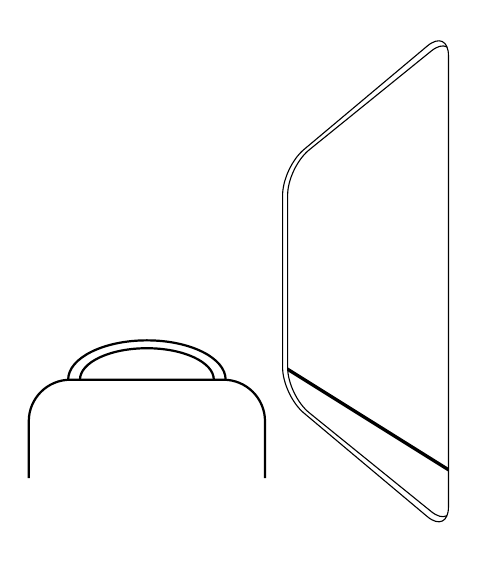
\begin{tikzpicture}[scale = 0.5]
		\draw[thick] (-2, -2.5) arc (180:0:2 and 1);
		\draw[thick] (-1.7, -2.5) arc (180:0: 1.7 and 0.8);
		\draw[thick, rounded corners = 15] (-3, -5) -- (-3, -2.5) -- (3, -2.5) -- (3, -5); 
		\draw[rounded corners = 10] (-40:4.5) -- (-40:10) -- (40:10) -- (40:4.5) -- cycle;
		\begin{scope}
    			\clip[rounded corners = 10] (-40:4.5) -- (-40:10) -- (40:10) -- (40:4.5) -- cycle;
			\draw[rounded corners = 10] (-39:4.6) -- (-39:10) -- (39:10) -- (39:4.6) -- cycle;
		\end{scope}
		\begin{scope}
    			\clip[rounded corners = 10] (-40:4.5) -- (-40:10) -- (40:10) -- (40:4.5) -- cycle;
			\clip[rounded corners = 10] (-39:4.6) -- (-39:10) -- (39:10) -- (39:4.6) -- cycle;
			\draw[very thick] (-32:0) -- (-32:13);
%			\fill[gray!80] (-32:0) -- (-32:13) -- (-50:13) -- cycle;
%			\fill[green!80!blue!60] (-32:0) -- (-32:13) -- (-15:13) -- cycle;
			\flash{1.13*7}{-1.13*3}{1.13*4}{thick}{0};
			\flash{0.91*7}{-0.91*3}{0.91*4}{thick}{1};
			\flash{0.71*7}{-0.71*3}{0.71*4}{thick}{2};
			\flash{0.55*7}{-0.55*3}{0.55*4}{thick}{3};
		\end{scope}
			\flash{1.13*7}{-1.13*3}{1.13*4}{thick, dashed}{0};
	\end{tikzpicture}	
	\end{minipage}
\end{figure}

	Фонарь $3$ ровно через \variants{секунду}{$1{,}5 секунды$} пересечет край щели и займет положение фонаря $0$. Кроме него за это время край щели пересекут еще фонари ($1$ и $2$). Тогда мальчик насчитает $3$ фонаря, кроме фонаря $0$, который уже посчитан ранее. Значит можно сказать, что мальчик насчитывает $\variants{3}{2}$ фонаря в секунду.
	
	 Аналогично будет выглядеть картина подсчета деревьев, только описанный процесс будет происходить не за $1$ секунду, а за $\variants{3}{4}$, и вместо $3$ фонарей мальчик будет видеть $\variants{4}{2}$ дерева в поле зрения. Тогда можно найти, что мальчик насчитывает $\variants{4}{2}$ дерева в $\variants{3}{4}$ секунды. А значит, насчитав \variants{$180$ фонарей}{$30$ деревьев}, он потратил $60$ секунд и насчитал \variants{$80$ деревьев}{$120$ фонарей}.

\olympanswer{\variants{$80$ деревьев.}{$120$ фонарей.}}	

\ifgrade
\begin{grade-env}
	\grade{5}{Предложен правильный механизм подсчета фонарей или деревьев.}
	\grade{2}{Найдено, что мальчик насчитывает $\variants{3}{2}$ фонаря в секунду.}
	\grade{2}{Найдено, что мальчик насчитывает $\variants{4}{2}$ дерева за $\variants{3}{4}$ секунды.}
	\grade{1}{Правильный ответ.}
\end{grade-env}
\fi